\subsection{Optimizing traditional data centers with renewable energy}
\label{sec:Comparison}

\hideit{
\begin{figure*}[!ht]
 \begin{center}
 \subfigure[Capacities]{{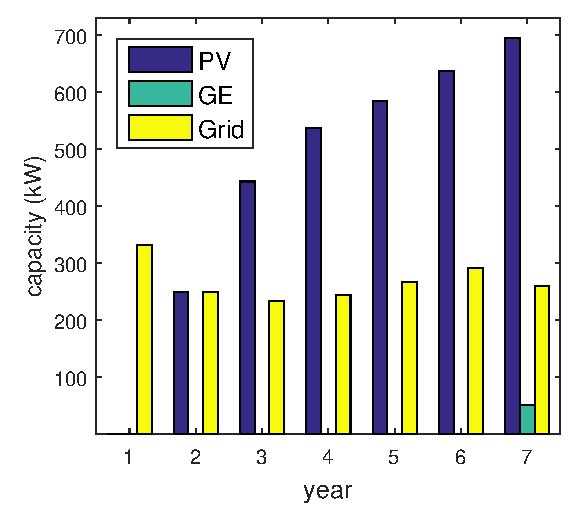
\includegraphics[width=0.32\columnwidth]{figs/long_term_capacity}}
 \label{f.capacity_annual_change}}
 \subfigure[Expenditures]{{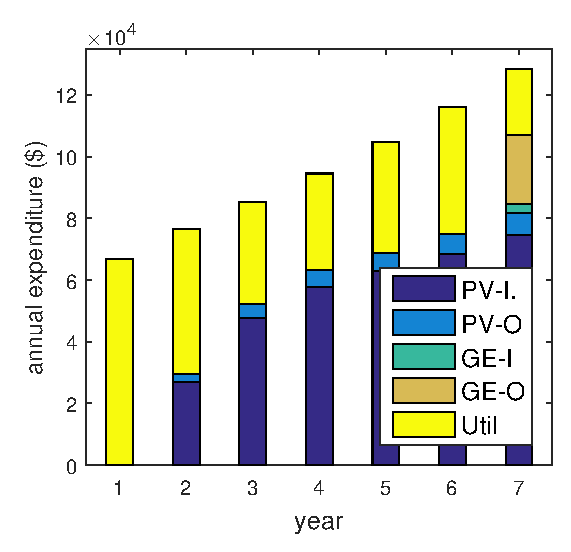
\includegraphics[width=0.32\columnwidth]{figs/long_term_cost}}
 \label{f.cost_annual_change}}
 \subfigure[Normalized emissions]{{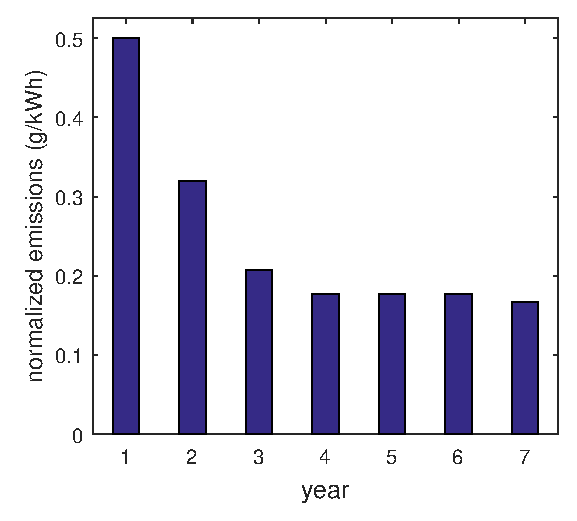
\includegraphics[width=0.32\columnwidth]{figs/long_term_co2_norm}}
 \label{f.co2_annual_change}} 

 \caption{Annual capacity planning. The data center is going to use more PV generation and GE generation while reducing the imported energy from the electricity grid. The major expenditure concentrates on the infrastructure of PV. The normalized emissions go down due to the high penetration of PV generation.}
 \label{f.annual_change}
 \end{center}

\end{figure*}
}
In this subsection, we evaluate the joint framework on planning and operating a sustainable data center. We answer three questions: How does the optimization framework plan annually? How much benefits can the optimization framework achieve? How do prediction errors impact on the proposed framework?

\textbf{Annual capacity planning.} In practice, the electricity prices, gas prices, and workload demand tend to increase in the long-term. The average annual-increasing rates of electricity prices, gas prices, and workload demand are $1.05$, $1.01$, and $1.09$ \cite{eiaElectricityPrices,gasPrice,StevenGlobalTraffic}. Meanwhile, the amortized cost of PV array decreases 12\% annually \cite{solarCost}.

Figure~\ref{f.capacity_annual_change} presents the capacities of power sources in 7 years. In general, the data center increases the capacity of PV annually but not the peak grid power consumption. In the first year, the data center prefers the electricity grid to other power sources because of the low electricity price. However, the data center significantly expands PV generation capacity from year 2 as the electricity prices increase and the infrastructure cost of PV decreases. In year 7, the data center provisions GE generation since the slow natural gas becomes relatively cheaper than the imported electricity. Although the data center prefers to use PV, the peak grid power consumption is still noticeably large. The intuition behind this is that PV generation is not available during night time which requires the data center to provision grid power.

Figure~\ref{f.cost_annual_change} shows the annual breakdown expenditures of the data center. In the first year, the utility bill (Util) of the imported energy from the electricity grid is dominant. Meanwhile, the cost of PV infrastructure (PV-I) quickly increases because PV amortized cost is added by installing more PV every year. The PV O\&M (PV-O) expenditure linearly increases as the PV capacity goes up. In year 7, the GE O\&M cost (GE-O) is 15\% the total annual expenditure. GE-O mainly comes from the amount of natural gas supplied to the GE.

The annually normalized emissions of the data center, defined as the ratios of total emissions to the total power demand, are plotted in Figure~\ref{f.co2_annual_change}. Since the normalized emissions of the electricity grid are high, the normalized emissions of the data center are highest in year 1.
The increase of the PV generation can reduce normalized emissions for the data center. The normalized emissions sharply go down to 36\% in year 4 as compared to the first year. However, there is little change from year 4 to year 7 as the ratio of PV capacity to other power sources is not considerably decreased.

\hideit{
\begin{figure*}[!ht]
 \begin{center}
	 \subfigure[Grid-only (GRID)]{{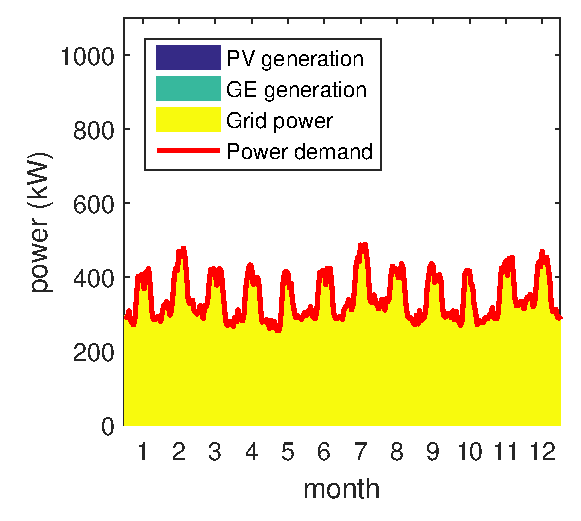
\includegraphics[width=0.32\columnwidth]{figs/nz-grid_year}}
	 \label{f.grid}}
	 \subfigure[Supply-only (SUP)]{{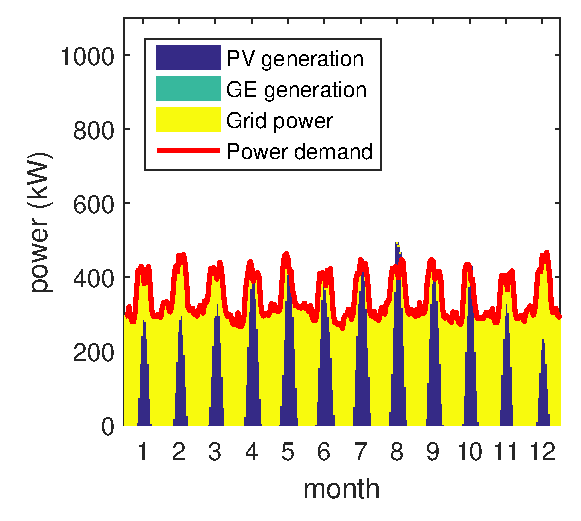
\includegraphics[width=0.32\columnwidth]{figs/nz-supply_year}}
	 \label{f.supply}}
	
	 \subfigure[Demand-only (DEM)]{{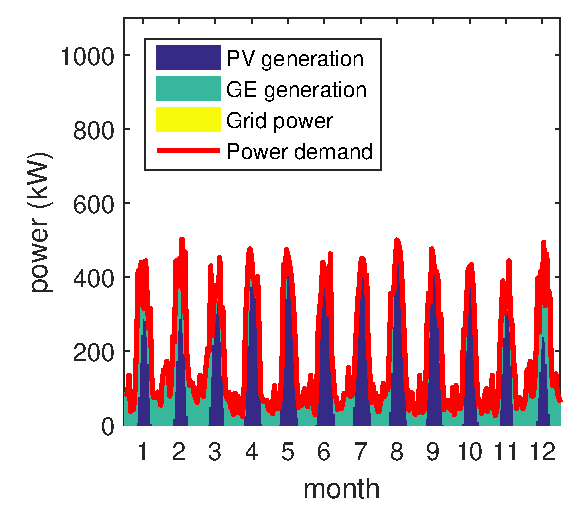
\includegraphics[width=0.32\columnwidth]{figs/nz-demand_year}}
	 \label{f.demand}}
	 \subfigure[Proposed (PROP)]{{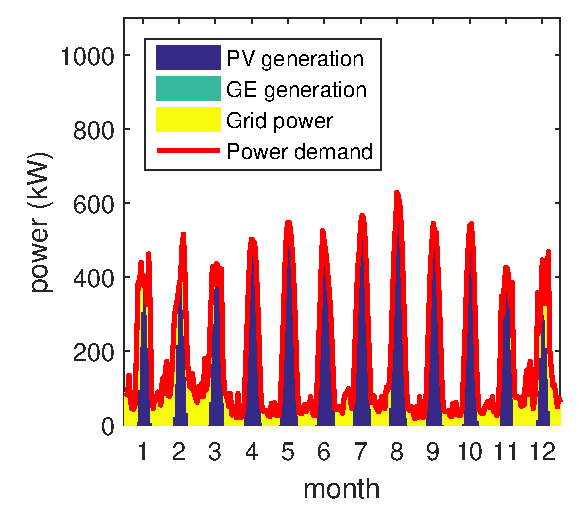
\includegraphics[width=0.32\columnwidth]{figs/nz-int_year}}
	 \label{f.integrated}}

 \caption{The power profiles of the baseline methods and the proposed framework in year 5. GRID provisions the only grid power. SUP optimizes the power sources only at the supply side. DEM optimizes the power demand, i.e., scheduling the batch jobs. } 
 \label{f.behaviors}
 \end{center} 

\end{figure*}
}

\textbf{How much cost savings and emission reductions does the proposed framework achieve?} To highlight the benefits of the proposed framework, we compare the proposed framework (PROP) with three baseline methods, namely grid-only, supply-only, and demand-only. 
\begin{itemize}

 \item Grid-only (GRID): \new{The grid-only method only uses the grid power from the electricity grid to provision the power demand. It does not use any power demand management techniques.}

 \item Supply-only (SUP): Given the power demand, the supply-only method optimizes capacity planning at the supply side.
This method can optimize the use of energy sources among PV, GE, and the public electricity grid. 

 \item Demand-only (DEM): \new{At the supply side, the capacities of PV and GE generation are set at 50\% and 70\% of the power demand capacity, respectively. 
The demand-only method optimizes the power demand, i.e., scheduling the batch jobs, to reduce the operational cost.}

\end{itemize}
In fact, PROP combines the SUP and DEM, and therefore can provide the best cost reductions.

The power profiles of these four methods in twelve typical days representing for the twelve months in year 5 are shown in Figure \ref{f.behaviors}.
GRID provisions power only from the electricity grid. SUP prefers the PV sources to the electricity grid and GE. Meanwhile, DEM utilizes installed GE generators because the electricity price is relatively more expensive than the O\&M cost of GE sources. However, PROP uses only PV generation and grid power. In Figure \ref{f.demand} and \ref{f.integrated}, DEM and PROP shape the power demand to follow the PV generation while GRID and SUP are dependent on imported electricity.
\hideit{
\begin{figure}[!th]
 \begin{center} 
 % \subfigure[Capacities]{{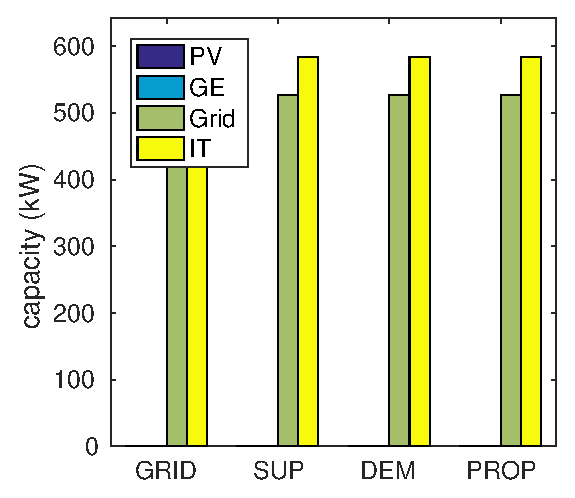
\includegraphics[width=0.48\columnwidth]{figs/capacity_comparison}}
 % \label{f.capacity_comp}}
 % \hspace{0.5cm}
 \subfigure[Expenditures]{{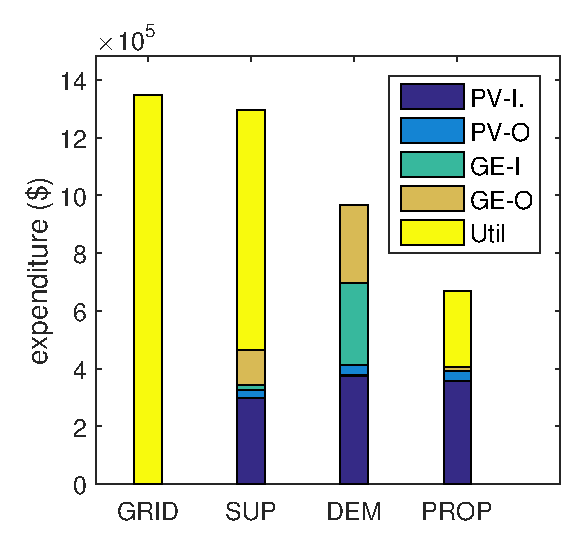
\includegraphics[width=0.32\columnwidth]{figs/cost_comparison}}
 \label{f.cost_comp}}
 % \hspace{0.5cm}
 \subfigure[Emissions]{{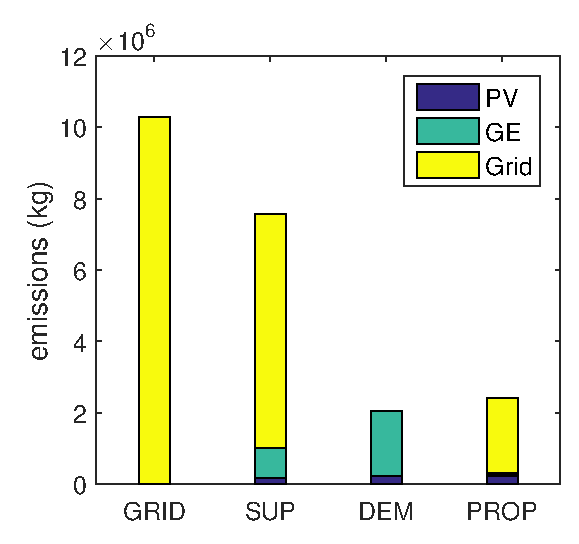
\includegraphics[width=0.32\columnwidth]{figs/emission_comparison}}
 \label{f.co2_comp}} 

 \caption{Comparisons with baseline methods. The proposed framework reduces up to 50\% of the total expenditures, and significantly cuts down 75\% greenhouse gas emissions.} 
 \label{f.basic}

 \end{center}
\end{figure}
}

We evaluate the four methods in terms of costs and emissions in Figure \ref{f.basic}. It shows that PROP remarkably reduces the total expenditure by 50\% while it achieves very close emissions to the lowest one, i.e., DEM. In Figure \ref{f.cost_comp}, SUP slightly reduces the total cost as it still depends much on the electricity grid. However, DEM shows that power management at demand side is very effective because it makes the power demand follow the PV generation.

\delete{\textbf{Should we provision IT capacity?} In order to highlight the importance of optimizing IT capacity, we carry out an experiment that plans the capacities of IT capacity and power sources. In Figure {\ref{f.IT}}, the IT capacities in the four methods are different. The proposed framework allows data center operators to provision the smallest IT capacity compared to other baseline methods. Consequently, the proposed framework can significantly reduce the total expenditure. Hence, the capacity of IT plays an important role reducing the total cost of ownership.}

\del{
	\begin{figure}[!htbp]
		\begin{center}
			\subfigure[Capacity]{{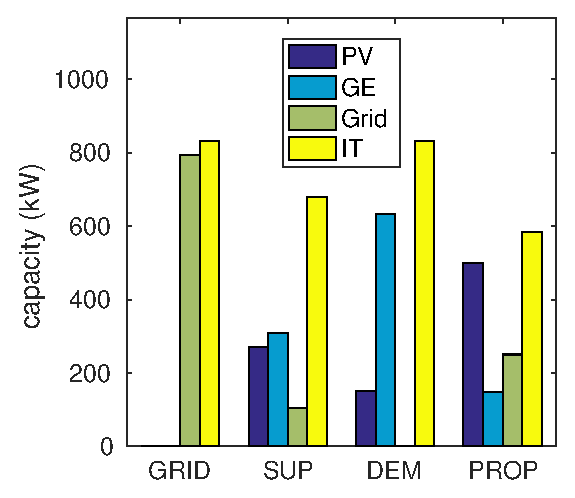
\includegraphics[width=0.48\columnwidth]{figs/capacity_IT}}
				\label{f.capacity_IT}}
			\subfigure[Cost]{{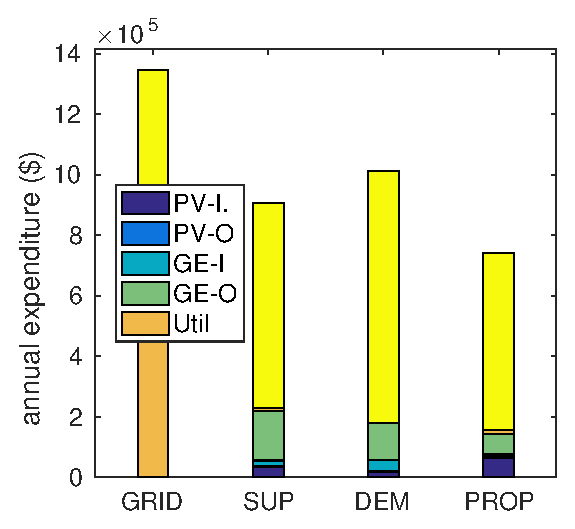
\includegraphics[width=0.48\columnwidth]{figs/cost_IT}}
				\label{f.cost_IT}}
			\caption{Comparisons with different baselines when IT capacity is also optimized. The IT capacitiy plays an important role in capacity planning.}
			\label{f.IT}
		\end{center}
	\end{figure}}


\textbf{\textit{Key insights}}: (i) The proposed framework not only remarkably reduce the total cost, but also utilizes renewable energy very well. (ii) As the renewable installation becomes more cost-effective, the proposed framework prefers to use renewable energy and reduce the dependence of sustainable data centers on the electricity grid. 
%\delete{(v) If we have opportunity to optimize IT subsystem, this can have considerate impact on the total annual expenditure of the data center.}